\documentclass{article} % For LaTeX2e
\usepackage{iclr2022_conference,times}
% Optional math commands from https://github.com/goodfeli/dlbook_notation.
%%%%% NEW MATH DEFINITIONS %%%%%

\usepackage{amsmath,amsfonts,bm}

% Mark sections of captions for referring to divisions of figures
\newcommand{\figleft}{{\em (Left)}}
\newcommand{\figcenter}{{\em (Center)}}
\newcommand{\figright}{{\em (Right)}}
\newcommand{\figtop}{{\em (Top)}}
\newcommand{\figbottom}{{\em (Bottom)}}
\newcommand{\captiona}{{\em (a)}}
\newcommand{\captionb}{{\em (b)}}
\newcommand{\captionc}{{\em (c)}}
\newcommand{\captiond}{{\em (d)}}

% Highlight a newly defined term
\newcommand{\newterm}[1]{{\bf #1}}


% Figure reference, lower-case.
\def\figref#1{figure~\ref{#1}}
% Figure reference, capital. For start of sentence
\def\Figref#1{Figure~\ref{#1}}
\def\twofigref#1#2{figures \ref{#1} and \ref{#2}}
\def\quadfigref#1#2#3#4{figures \ref{#1}, \ref{#2}, \ref{#3} and \ref{#4}}
% Section reference, lower-case.
\def\secref#1{section~\ref{#1}}
% Section reference, capital.
\def\Secref#1{Section~\ref{#1}}
% Reference to two sections.
\def\twosecrefs#1#2{sections \ref{#1} and \ref{#2}}
% Reference to three sections.
\def\secrefs#1#2#3{sections \ref{#1}, \ref{#2} and \ref{#3}}
% Reference to an equation, lower-case.
\def\eqref#1{equation~\ref{#1}}
% Reference to an equation, upper case
\def\Eqref#1{Equation~\ref{#1}}
% A raw reference to an equation---avoid using if possible
\def\plaineqref#1{\ref{#1}}
% Reference to a chapter, lower-case.
\def\chapref#1{chapter~\ref{#1}}
% Reference to an equation, upper case.
\def\Chapref#1{Chapter~\ref{#1}}
% Reference to a range of chapters
\def\rangechapref#1#2{chapters\ref{#1}--\ref{#2}}
% Reference to an algorithm, lower-case.
\def\algref#1{algorithm~\ref{#1}}
% Reference to an algorithm, upper case.
\def\Algref#1{Algorithm~\ref{#1}}
\def\twoalgref#1#2{algorithms \ref{#1} and \ref{#2}}
\def\Twoalgref#1#2{Algorithms \ref{#1} and \ref{#2}}
% Reference to a part, lower case
\def\partref#1{part~\ref{#1}}
% Reference to a part, upper case
\def\Partref#1{Part~\ref{#1}}
\def\twopartref#1#2{parts \ref{#1} and \ref{#2}}

\def\ceil#1{\lceil #1 \rceil}
\def\floor#1{\lfloor #1 \rfloor}
\def\1{\bm{1}}
\newcommand{\train}{\mathcal{D}}
\newcommand{\valid}{\mathcal{D_{\mathrm{valid}}}}
\newcommand{\test}{\mathcal{D_{\mathrm{test}}}}

\def\eps{{\epsilon}}


% Random variables
\def\reta{{\textnormal{$\eta$}}}
\def\ra{{\textnormal{a}}}
\def\rb{{\textnormal{b}}}
\def\rc{{\textnormal{c}}}
\def\rd{{\textnormal{d}}}
\def\re{{\textnormal{e}}}
\def\rf{{\textnormal{f}}}
\def\rg{{\textnormal{g}}}
\def\rh{{\textnormal{h}}}
\def\ri{{\textnormal{i}}}
\def\rj{{\textnormal{j}}}
\def\rk{{\textnormal{k}}}
\def\rl{{\textnormal{l}}}
% rm is already a command, just don't name any random variables m
\def\rn{{\textnormal{n}}}
\def\ro{{\textnormal{o}}}
\def\rp{{\textnormal{p}}}
\def\rq{{\textnormal{q}}}
\def\rr{{\textnormal{r}}}
\def\rs{{\textnormal{s}}}
\def\rt{{\textnormal{t}}}
\def\ru{{\textnormal{u}}}
\def\rv{{\textnormal{v}}}
\def\rw{{\textnormal{w}}}
\def\rx{{\textnormal{x}}}
\def\ry{{\textnormal{y}}}
\def\rz{{\textnormal{z}}}

% Random vectors
\def\rvepsilon{{\mathbf{\epsilon}}}
\def\rvtheta{{\mathbf{\theta}}}
\def\rva{{\mathbf{a}}}
\def\rvb{{\mathbf{b}}}
\def\rvc{{\mathbf{c}}}
\def\rvd{{\mathbf{d}}}
\def\rve{{\mathbf{e}}}
\def\rvf{{\mathbf{f}}}
\def\rvg{{\mathbf{g}}}
\def\rvh{{\mathbf{h}}}
\def\rvu{{\mathbf{i}}}
\def\rvj{{\mathbf{j}}}
\def\rvk{{\mathbf{k}}}
\def\rvl{{\mathbf{l}}}
\def\rvm{{\mathbf{m}}}
\def\rvn{{\mathbf{n}}}
\def\rvo{{\mathbf{o}}}
\def\rvp{{\mathbf{p}}}
\def\rvq{{\mathbf{q}}}
\def\rvr{{\mathbf{r}}}
\def\rvs{{\mathbf{s}}}
\def\rvt{{\mathbf{t}}}
\def\rvu{{\mathbf{u}}}
\def\rvv{{\mathbf{v}}}
\def\rvw{{\mathbf{w}}}
\def\rvx{{\mathbf{x}}}
\def\rvy{{\mathbf{y}}}
\def\rvz{{\mathbf{z}}}

% Elements of random vectors
\def\erva{{\textnormal{a}}}
\def\ervb{{\textnormal{b}}}
\def\ervc{{\textnormal{c}}}
\def\ervd{{\textnormal{d}}}
\def\erve{{\textnormal{e}}}
\def\ervf{{\textnormal{f}}}
\def\ervg{{\textnormal{g}}}
\def\ervh{{\textnormal{h}}}
\def\ervi{{\textnormal{i}}}
\def\ervj{{\textnormal{j}}}
\def\ervk{{\textnormal{k}}}
\def\ervl{{\textnormal{l}}}
\def\ervm{{\textnormal{m}}}
\def\ervn{{\textnormal{n}}}
\def\ervo{{\textnormal{o}}}
\def\ervp{{\textnormal{p}}}
\def\ervq{{\textnormal{q}}}
\def\ervr{{\textnormal{r}}}
\def\ervs{{\textnormal{s}}}
\def\ervt{{\textnormal{t}}}
\def\ervu{{\textnormal{u}}}
\def\ervv{{\textnormal{v}}}
\def\ervw{{\textnormal{w}}}
\def\ervx{{\textnormal{x}}}
\def\ervy{{\textnormal{y}}}
\def\ervz{{\textnormal{z}}}

% Random matrices
\def\rmA{{\mathbf{A}}}
\def\rmB{{\mathbf{B}}}
\def\rmC{{\mathbf{C}}}
\def\rmD{{\mathbf{D}}}
\def\rmE{{\mathbf{E}}}
\def\rmF{{\mathbf{F}}}
\def\rmG{{\mathbf{G}}}
\def\rmH{{\mathbf{H}}}
\def\rmI{{\mathbf{I}}}
\def\rmJ{{\mathbf{J}}}
\def\rmK{{\mathbf{K}}}
\def\rmL{{\mathbf{L}}}
\def\rmM{{\mathbf{M}}}
\def\rmN{{\mathbf{N}}}
\def\rmO{{\mathbf{O}}}
\def\rmP{{\mathbf{P}}}
\def\rmQ{{\mathbf{Q}}}
\def\rmR{{\mathbf{R}}}
\def\rmS{{\mathbf{S}}}
\def\rmT{{\mathbf{T}}}
\def\rmU{{\mathbf{U}}}
\def\rmV{{\mathbf{V}}}
\def\rmW{{\mathbf{W}}}
\def\rmX{{\mathbf{X}}}
\def\rmY{{\mathbf{Y}}}
\def\rmZ{{\mathbf{Z}}}

% Elements of random matrices
\def\ermA{{\textnormal{A}}}
\def\ermB{{\textnormal{B}}}
\def\ermC{{\textnormal{C}}}
\def\ermD{{\textnormal{D}}}
\def\ermE{{\textnormal{E}}}
\def\ermF{{\textnormal{F}}}
\def\ermG{{\textnormal{G}}}
\def\ermH{{\textnormal{H}}}
\def\ermI{{\textnormal{I}}}
\def\ermJ{{\textnormal{J}}}
\def\ermK{{\textnormal{K}}}
\def\ermL{{\textnormal{L}}}
\def\ermM{{\textnormal{M}}}
\def\ermN{{\textnormal{N}}}
\def\ermO{{\textnormal{O}}}
\def\ermP{{\textnormal{P}}}
\def\ermQ{{\textnormal{Q}}}
\def\ermR{{\textnormal{R}}}
\def\ermS{{\textnormal{S}}}
\def\ermT{{\textnormal{T}}}
\def\ermU{{\textnormal{U}}}
\def\ermV{{\textnormal{V}}}
\def\ermW{{\textnormal{W}}}
\def\ermX{{\textnormal{X}}}
\def\ermY{{\textnormal{Y}}}
\def\ermZ{{\textnormal{Z}}}

% Vectors
\def\vzero{{\bm{0}}}
\def\vone{{\bm{1}}}
\def\vmu{{\bm{\mu}}}
\def\vtheta{{\bm{\theta}}}
\def\va{{\bm{a}}}
\def\vb{{\bm{b}}}
\def\vc{{\bm{c}}}
\def\vd{{\bm{d}}}
\def\ve{{\bm{e}}}
\def\vf{{\bm{f}}}
\def\vg{{\bm{g}}}
\def\vh{{\bm{h}}}
\def\vi{{\bm{i}}}
\def\vj{{\bm{j}}}
\def\vk{{\bm{k}}}
\def\vl{{\bm{l}}}
\def\vm{{\bm{m}}}
\def\vn{{\bm{n}}}
\def\vo{{\bm{o}}}
\def\vp{{\bm{p}}}
\def\vq{{\bm{q}}}
\def\vr{{\bm{r}}}
\def\vs{{\bm{s}}}
\def\vt{{\bm{t}}}
\def\vu{{\bm{u}}}
\def\vv{{\bm{v}}}
\def\vw{{\bm{w}}}
\def\vx{{\bm{x}}}
\def\vy{{\bm{y}}}
\def\vz{{\bm{z}}}

% Elements of vectors
\def\evalpha{{\alpha}}
\def\evbeta{{\beta}}
\def\evepsilon{{\epsilon}}
\def\evlambda{{\lambda}}
\def\evomega{{\omega}}
\def\evmu{{\mu}}
\def\evpsi{{\psi}}
\def\evsigma{{\sigma}}
\def\evtheta{{\theta}}
\def\eva{{a}}
\def\evb{{b}}
\def\evc{{c}}
\def\evd{{d}}
\def\eve{{e}}
\def\evf{{f}}
\def\evg{{g}}
\def\evh{{h}}
\def\evi{{i}}
\def\evj{{j}}
\def\evk{{k}}
\def\evl{{l}}
\def\evm{{m}}
\def\evn{{n}}
\def\evo{{o}}
\def\evp{{p}}
\def\evq{{q}}
\def\evr{{r}}
\def\evs{{s}}
\def\evt{{t}}
\def\evu{{u}}
\def\evv{{v}}
\def\evw{{w}}
\def\evx{{x}}
\def\evy{{y}}
\def\evz{{z}}

% Matrix
\def\mA{{\bm{A}}}
\def\mB{{\bm{B}}}
\def\mC{{\bm{C}}}
\def\mD{{\bm{D}}}
\def\mE{{\bm{E}}}
\def\mF{{\bm{F}}}
\def\mG{{\bm{G}}}
\def\mH{{\bm{H}}}
\def\mI{{\bm{I}}}
\def\mJ{{\bm{J}}}
\def\mK{{\bm{K}}}
\def\mL{{\bm{L}}}
\def\mM{{\bm{M}}}
\def\mN{{\bm{N}}}
\def\mO{{\bm{O}}}
\def\mP{{\bm{P}}}
\def\mQ{{\bm{Q}}}
\def\mR{{\bm{R}}}
\def\mS{{\bm{S}}}
\def\mT{{\bm{T}}}
\def\mU{{\bm{U}}}
\def\mV{{\bm{V}}}
\def\mW{{\bm{W}}}
\def\mX{{\bm{X}}}
\def\mY{{\bm{Y}}}
\def\mZ{{\bm{Z}}}
\def\mBeta{{\bm{\beta}}}
\def\mPhi{{\bm{\Phi}}}
\def\mLambda{{\bm{\Lambda}}}
\def\mSigma{{\bm{\Sigma}}}

% Tensor
\DeclareMathAlphabet{\mathsfit}{\encodingdefault}{\sfdefault}{m}{sl}
\SetMathAlphabet{\mathsfit}{bold}{\encodingdefault}{\sfdefault}{bx}{n}
\newcommand{\tens}[1]{\bm{\mathsfit{#1}}}
\def\tA{{\tens{A}}}
\def\tB{{\tens{B}}}
\def\tC{{\tens{C}}}
\def\tD{{\tens{D}}}
\def\tE{{\tens{E}}}
\def\tF{{\tens{F}}}
\def\tG{{\tens{G}}}
\def\tH{{\tens{H}}}
\def\tI{{\tens{I}}}
\def\tJ{{\tens{J}}}
\def\tK{{\tens{K}}}
\def\tL{{\tens{L}}}
\def\tM{{\tens{M}}}
\def\tN{{\tens{N}}}
\def\tO{{\tens{O}}}
\def\tP{{\tens{P}}}
\def\tQ{{\tens{Q}}}
\def\tR{{\tens{R}}}
\def\tS{{\tens{S}}}
\def\tT{{\tens{T}}}
\def\tU{{\tens{U}}}
\def\tV{{\tens{V}}}
\def\tW{{\tens{W}}}
\def\tX{{\tens{X}}}
\def\tY{{\tens{Y}}}
\def\tZ{{\tens{Z}}}


% Graph
\def\gA{{\mathcal{A}}}
\def\gB{{\mathcal{B}}}
\def\gC{{\mathcal{C}}}
\def\gD{{\mathcal{D}}}
\def\gE{{\mathcal{E}}}
\def\gF{{\mathcal{F}}}
\def\gG{{\mathcal{G}}}
\def\gH{{\mathcal{H}}}
\def\gI{{\mathcal{I}}}
\def\gJ{{\mathcal{J}}}
\def\gK{{\mathcal{K}}}
\def\gL{{\mathcal{L}}}
\def\gM{{\mathcal{M}}}
\def\gN{{\mathcal{N}}}
\def\gO{{\mathcal{O}}}
\def\gP{{\mathcal{P}}}
\def\gQ{{\mathcal{Q}}}
\def\gR{{\mathcal{R}}}
\def\gS{{\mathcal{S}}}
\def\gT{{\mathcal{T}}}
\def\gU{{\mathcal{U}}}
\def\gV{{\mathcal{V}}}
\def\gW{{\mathcal{W}}}
\def\gX{{\mathcal{X}}}
\def\gY{{\mathcal{Y}}}
\def\gZ{{\mathcal{Z}}}

% Sets
\def\sA{{\mathbb{A}}}
\def\sB{{\mathbb{B}}}
\def\sC{{\mathbb{C}}}
\def\sD{{\mathbb{D}}}
% Don't use a set called E, because this would be the same as our symbol
% for expectation.
\def\sF{{\mathbb{F}}}
\def\sG{{\mathbb{G}}}
\def\sH{{\mathbb{H}}}
\def\sI{{\mathbb{I}}}
\def\sJ{{\mathbb{J}}}
\def\sK{{\mathbb{K}}}
\def\sL{{\mathbb{L}}}
\def\sM{{\mathbb{M}}}
\def\sN{{\mathbb{N}}}
\def\sO{{\mathbb{O}}}
\def\sP{{\mathbb{P}}}
\def\sQ{{\mathbb{Q}}}
\def\sR{{\mathbb{R}}}
\def\sS{{\mathbb{S}}}
\def\sT{{\mathbb{T}}}
\def\sU{{\mathbb{U}}}
\def\sV{{\mathbb{V}}}
\def\sW{{\mathbb{W}}}
\def\sX{{\mathbb{X}}}
\def\sY{{\mathbb{Y}}}
\def\sZ{{\mathbb{Z}}}

% Entries of a matrix
\def\emLambda{{\Lambda}}
\def\emA{{A}}
\def\emB{{B}}
\def\emC{{C}}
\def\emD{{D}}
\def\emE{{E}}
\def\emF{{F}}
\def\emG{{G}}
\def\emH{{H}}
\def\emI{{I}}
\def\emJ{{J}}
\def\emK{{K}}
\def\emL{{L}}
\def\emM{{M}}
\def\emN{{N}}
\def\emO{{O}}
\def\emP{{P}}
\def\emQ{{Q}}
\def\emR{{R}}
\def\emS{{S}}
\def\emT{{T}}
\def\emU{{U}}
\def\emV{{V}}
\def\emW{{W}}
\def\emX{{X}}
\def\emY{{Y}}
\def\emZ{{Z}}
\def\emSigma{{\Sigma}}

% entries of a tensor
% Same font as tensor, without \bm wrapper
\newcommand{\etens}[1]{\mathsfit{#1}}
\def\etLambda{{\etens{\Lambda}}}
\def\etA{{\etens{A}}}
\def\etB{{\etens{B}}}
\def\etC{{\etens{C}}}
\def\etD{{\etens{D}}}
\def\etE{{\etens{E}}}
\def\etF{{\etens{F}}}
\def\etG{{\etens{G}}}
\def\etH{{\etens{H}}}
\def\etI{{\etens{I}}}
\def\etJ{{\etens{J}}}
\def\etK{{\etens{K}}}
\def\etL{{\etens{L}}}
\def\etM{{\etens{M}}}
\def\etN{{\etens{N}}}
\def\etO{{\etens{O}}}
\def\etP{{\etens{P}}}
\def\etQ{{\etens{Q}}}
\def\etR{{\etens{R}}}
\def\etS{{\etens{S}}}
\def\etT{{\etens{T}}}
\def\etU{{\etens{U}}}
\def\etV{{\etens{V}}}
\def\etW{{\etens{W}}}
\def\etX{{\etens{X}}}
\def\etY{{\etens{Y}}}
\def\etZ{{\etens{Z}}}

% The true underlying data generating distribution
\newcommand{\pdata}{p_{\rm{data}}}
% The empirical distribution defined by the training set
\newcommand{\ptrain}{\hat{p}_{\rm{data}}}
\newcommand{\Ptrain}{\hat{P}_{\rm{data}}}
% The model distribution
\newcommand{\pmodel}{p_{\rm{model}}}
\newcommand{\Pmodel}{P_{\rm{model}}}
\newcommand{\ptildemodel}{\tilde{p}_{\rm{model}}}
% Stochastic autoencoder distributions
\newcommand{\pencode}{p_{\rm{encoder}}}
\newcommand{\pdecode}{p_{\rm{decoder}}}
\newcommand{\precons}{p_{\rm{reconstruct}}}

\newcommand{\laplace}{\mathrm{Laplace}} % Laplace distribution

\newcommand{\E}{\mathbb{E}}
\newcommand{\Ls}{\mathcal{L}}
\newcommand{\R}{\mathbb{R}}
\newcommand{\emp}{\tilde{p}}
\newcommand{\lr}{\alpha}
\newcommand{\reg}{\lambda}
\newcommand{\rect}{\mathrm{rectifier}}
\newcommand{\softmax}{\mathrm{softmax}}
\newcommand{\sigmoid}{\sigma}
\newcommand{\softplus}{\zeta}
\newcommand{\KL}{D_{\mathrm{KL}}}
\newcommand{\Var}{\mathrm{Var}}
\newcommand{\standarderror}{\mathrm{SE}}
\newcommand{\Cov}{\mathrm{Cov}}
% Wolfram Mathworld says $L^2$ is for function spaces and $\ell^2$ is for vectors
% But then they seem to use $L^2$ for vectors throughout the site, and so does
% wikipedia.
\newcommand{\normlzero}{L^0}
\newcommand{\normlone}{L^1}
\newcommand{\normltwo}{L^2}
\newcommand{\normlp}{L^p}
\newcommand{\normmax}{L^\infty}

\newcommand{\parents}{Pa} % See usage in notation.tex. Chosen to match Daphne's book.

\DeclareMathOperator*{\argmax}{arg\,max}
\DeclareMathOperator*{\argmin}{arg\,min}

\DeclareMathOperator{\sign}{sign}
\DeclareMathOperator{\Tr}{Tr}
\let\ab\allowbreak


%######## APS360: Uncomment your submission name
\newcommand{\apsname}{Project Proposal}
%\newcommand{\apsname}{Progress Report}
%\newcommand{\apsname}{Final Report}

%######## APS360: Put your Group Number here
\newcommand{\gpnumber}{18}

\usepackage{hyperref}
\usepackage{url}
\usepackage{graphicx}
\usepackage{multicol}
\usepackage{caption}
\usepackage{hyperref}
\usepackage{longtable}

%######## APS360: Put your project Title here
\title{Object Detection and Depth Perception System for Visually Impaired People (AwareAI)
}


%######## APS360: Put your names, student IDs and Emails here
\author{Rick Lin  \\
Student\# 1007977076\\
\texttt{rick.lin@mail.utoronto.ca} \\
\And
Ruichen (Spencer) Li  \\
Student\# 1007623831 \\
\texttt{spencer.li@mail.utoronto.ca  } \\
\AND
Jason Tai  \\
Student\# 1008122363 \\
\texttt{jason.tai@mail.utoronto.ca} \\
\And 
\hspace{1.61cm} Danjie Tang \\
\hspace{1.61cm} Student\# 1008008941 \\
\hspace{1.61cm} \texttt{danjie.tang@mail.utoronto.ca}
}

% The \author macro works with any number of authors. There are two commands
% used to separate the names and addresses of multiple authors: \And and \AND.
%
% Using \And between authors leaves it to \LaTeX{} to determine where to break
% the lines. Using \AND forces a linebreak at that point. So, if \LaTeX{}
% puts 3 of 4 authors names on the first line, and the last on the second
% line, try using \AND instead of \And before the third author name.

\newcommand{\fix}{\marginpar{FIX}}
\newcommand{\new}{\marginpar{NEW}}

\iclrfinalcopy 
%######## APS360: Document starts here
\begin{document}


\maketitle

\begin{abstract}
Object detection and depth perception problems have been challenging and widely discussed for several years. With the advancements in deep neural networks (DNNs) and computer vision algorithms, there is a growing focus on refining learning strategies, model architectures, and their practical applications. In this paper, we propose AwareAI: an Object Detection and Depth Perception System for Visually Impaired People. Our system combines deep learning frameworks and a machine learning system with voice output to assist visually impaired individuals by providing information about the objects and obstacles in their view. By taking images as input, the system generates audio outputs that offer information about objects or obstacles in front of the user, including their distances. We utilize the NYU Depth V2 and ScanNet datasets to train the depth perception model and generate a depth map, and the ImageNet dataset to train the object detection model. We employ a support vector machine as our baseline model and make comparisons with our proposed deep learning model. Additionally, we present a comprehensive table outlining tasks, team members, deadlines, and a detailed project timeline. Collaboration methods and potential risks associated with the project are also discussed.

%######## APS360: Do not change the next line. This shows your Main body page count.
----Total Pages: \pageref{last_page}
\end{abstract}



%%%%%%%%%%%%%%%%%%%%% Start of Section 1: Intro %%%%%%%%%%%%%%%%%%%%%



\section{Introduction}
Many people around the world suffer from visual impairments and eye conditions, such as blurred vision, diabetic retinopathy, age-related macular degeneration, and other vision problems \cite{Types_of_Vision_Problems} . However, treatments for these visual impairments and eye conditions may not be accessible to everyone, and having constant assistance may not always be feasible. Without treatment or assistance, visually impaired individuals face a greater risk of injury due to collisions with obstacles like furniture, tripping on objects on the ground, or falling down stairs that they may not have seen. Our project, AwareAI, aims to address this issue.

AwareAI will assist the visually impaired by utilizing their smartphone camera, which is a relatively accessible tool, to record their environment and receive voice outputs about nearby objects and obstacles along with their respective distances. For example, the system may say, "There is a chair two meters away on your left." This will enable users to be more aware of their surroundings, thereby reducing the risk of collisions, tripping, and falling.

Deep learning is a suitable approach for developing this project because it is highly effective in object classification within images. Additionally, to ensure accessibility to as many people as possible, we will utilize only a single camera and refrain from using multiple cameras or LiDAR technology. Our model will take one picture at a time as input and accurately estimate distances using deep learning frameworks.


%%%%%%%%%%%%%%%%%%%%% Start of Section 2: Backgound and Related Work %%%%%%%%%%%%%%%%%%%%%



\section{Background and Related Work}

Several recent projects and studies have investigated both object detection and depth perception under different settings. Broadly, these approaches can be grouped into two categories. The first group of them relies on mathematical models and relationships. For example, they use known geometry information such as the size of the object in real life and compute the distance in between with mathematical formulas. Another kind of approach is learning-based, where most effort is spent on designing machine learning architectures and training a model that detects objects and estimates depths.


\subsection{ Triangle similarity for Object/Marker to Camera Distance}


\cite{PyImage_Triangle} proposes an approach that assumes the availability of external information, such as the object's dimensions and the camera's focal length. Upon receiving the image, this approach utilizes a pre-trained model to detect the object's edges and subsequently calculates the object's width in pixels within the image (Figure  \ref{triaSimi}). A relationship is then established between the real width of the object ($\displaystyle W$), the focal length ($\displaystyle F$), the object's width in the image ($\displaystyle P$), and the distance between the object and the camera ($\displaystyle D$) as follows:

\begin{equation}
\label{eqn: 1}
F = (P*D)/W
\end{equation}

% To cite images just copy and paste these

\begin{figure}[h]
\begin{center}
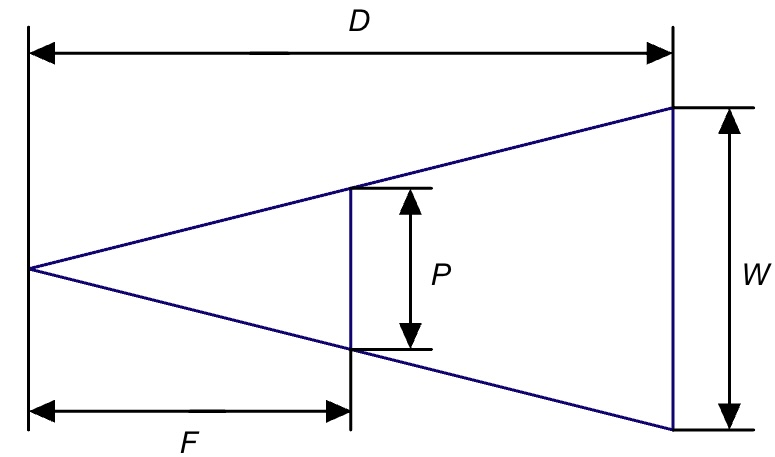
\includegraphics[width=0.3\textwidth]{Figs/triaSimi.png}
\end{center}
\caption{Geometric meaning of Equation \ref{eqn: 1}}
\label{triaSimi}
\end{figure}
%%%%%%%%%%%%%%%%%%%%%%

This method produces an estimation of 2.92 feet for an object located 3 feet away from the camera. However, this approach is flawed as its assumption regarding the availability of external information may not always be valid.

\subsection{Perception with Deep Learning and Low-cost Sensors}

\cite{Bauer2020} examines the feasibility of employing low-cost sensors to assist visually impaired individuals in comprehending their surroundings. The research group's system primarily comprises three components: local sensors, a remote server, and an output device, as illustrated in Figure \ref{Bauer2020-figure}.

% To cite images just copy and paste these
\begin{minipage}{.5\textwidth}
    \centering
    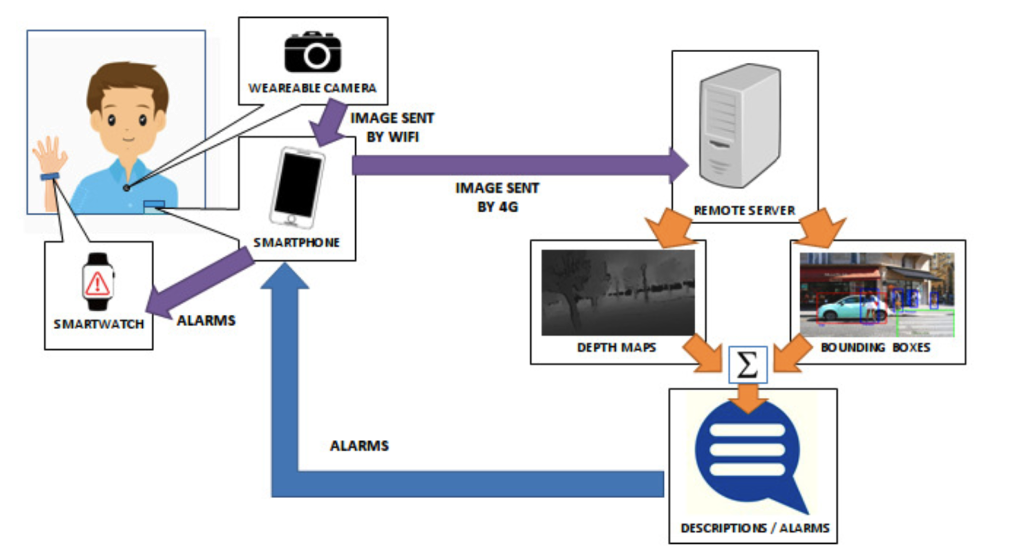
\includegraphics[height=3.8cm]{Figs/bauer-sensor.png}
    \captionof{figure}{Architecture of the system proposed by \citet{Bauer2020}}
    \label{Bauer2020-figure}
\end{minipage}
\begin{minipage}{.5\textwidth}
    \centering
    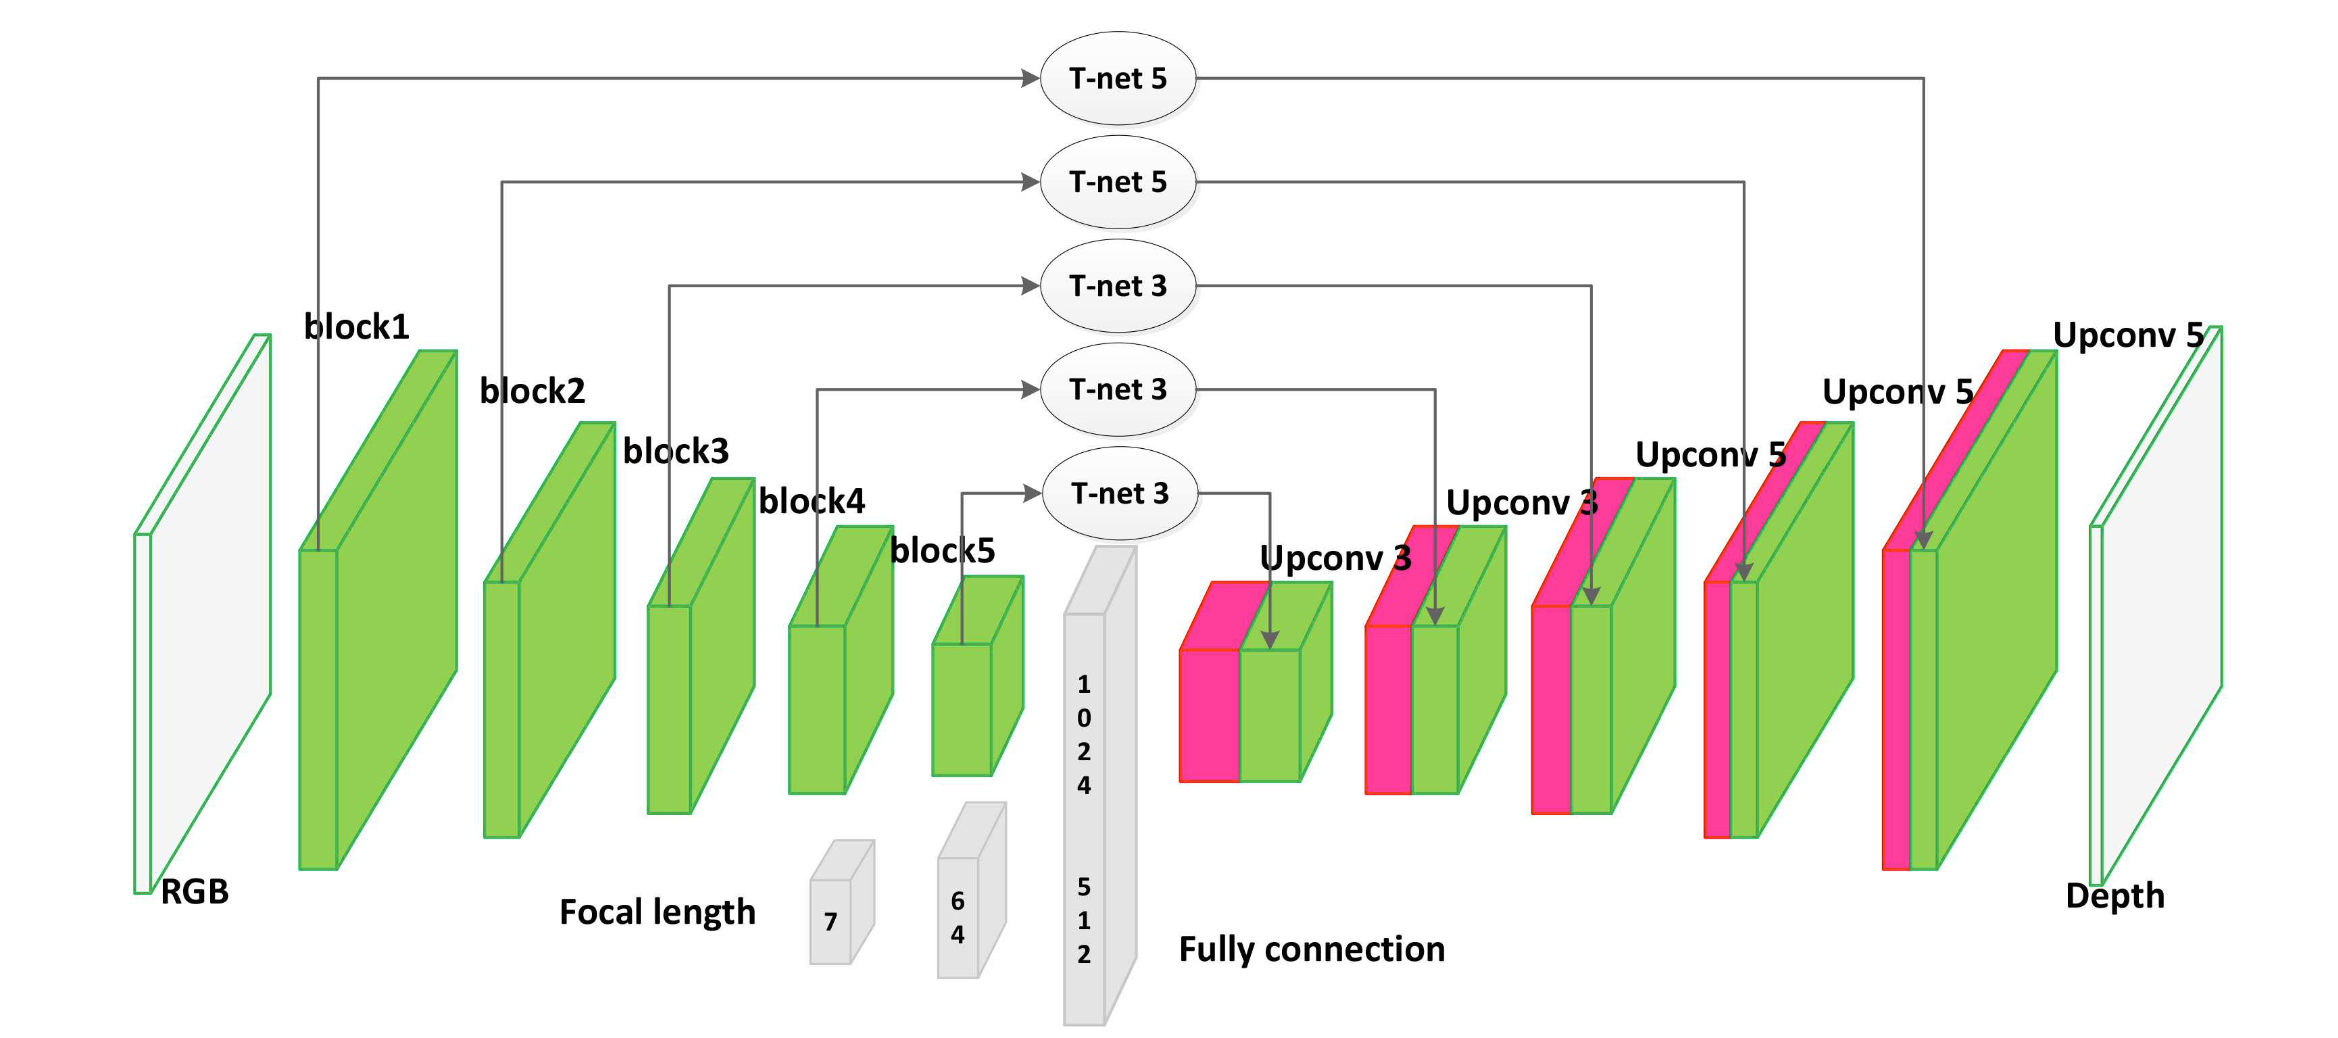
\includegraphics[height=3.8cm]{Figs/FocalDLPicAr.png}
    \captionof{figure}{Architecture introduced by \cite{FocalDL} where focal length is taken as an input}
    \label{FocalDLPicAr}
\end{minipage}
% \begin{figure}[h]
% \begin{center}
% 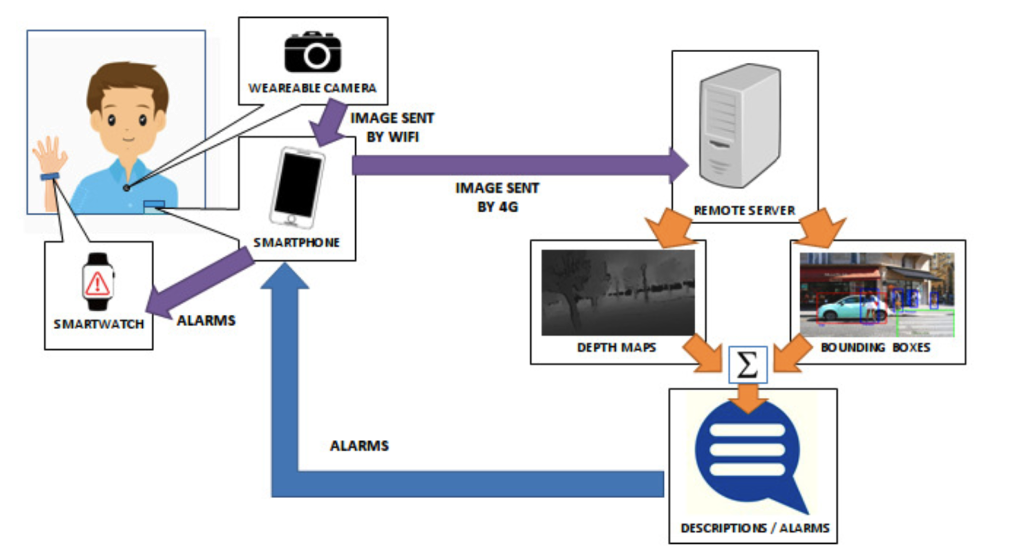
\includegraphics[width=0.6\textwidth]{Figs/bauer-sensor.png}
% \end{center}
% \caption{Architecture of the system proposed by \citet{Bauer2020}}
% \label{Bauer2020-figure}
% \end{figure}
%%%%%%%%%%%%%%%%%%%%%%

This system captures an image using a wearable camera and transmits it to users' smartphones, which then send the image to a remote server. On the remote server, the image is processed by a deep neural network (DNN) based on \cite{He2015}. The network generates a depth map and an annotated image where detected objects are enclosed within bounding boxes. The depth map and annotated image are combined to calculate depth information for each detected object. The results are then sent back to users' smartphones, where descriptions and alarms are generated. This system achieves a detection rate of 87.99 for obstacles.


\subsection{Depth Perception with know focal length}


\cite{FocalDL} addresses depth perception by incorporating the focal length of the camera into their end-to-end trained deep neural network (DNN). They opt to include the focal length as an input to the model, aiming to enhance the accuracy of their depth estimation. Figure \ref{FocalDLPicAr} illustrates the architecture of their approach, with the convolutional neural network (CNN) based on the VGG model proposed by \cite{VGG}.


% To cite images just copy and paste these
% \begin{figure}[h]
% \begin{center}
% 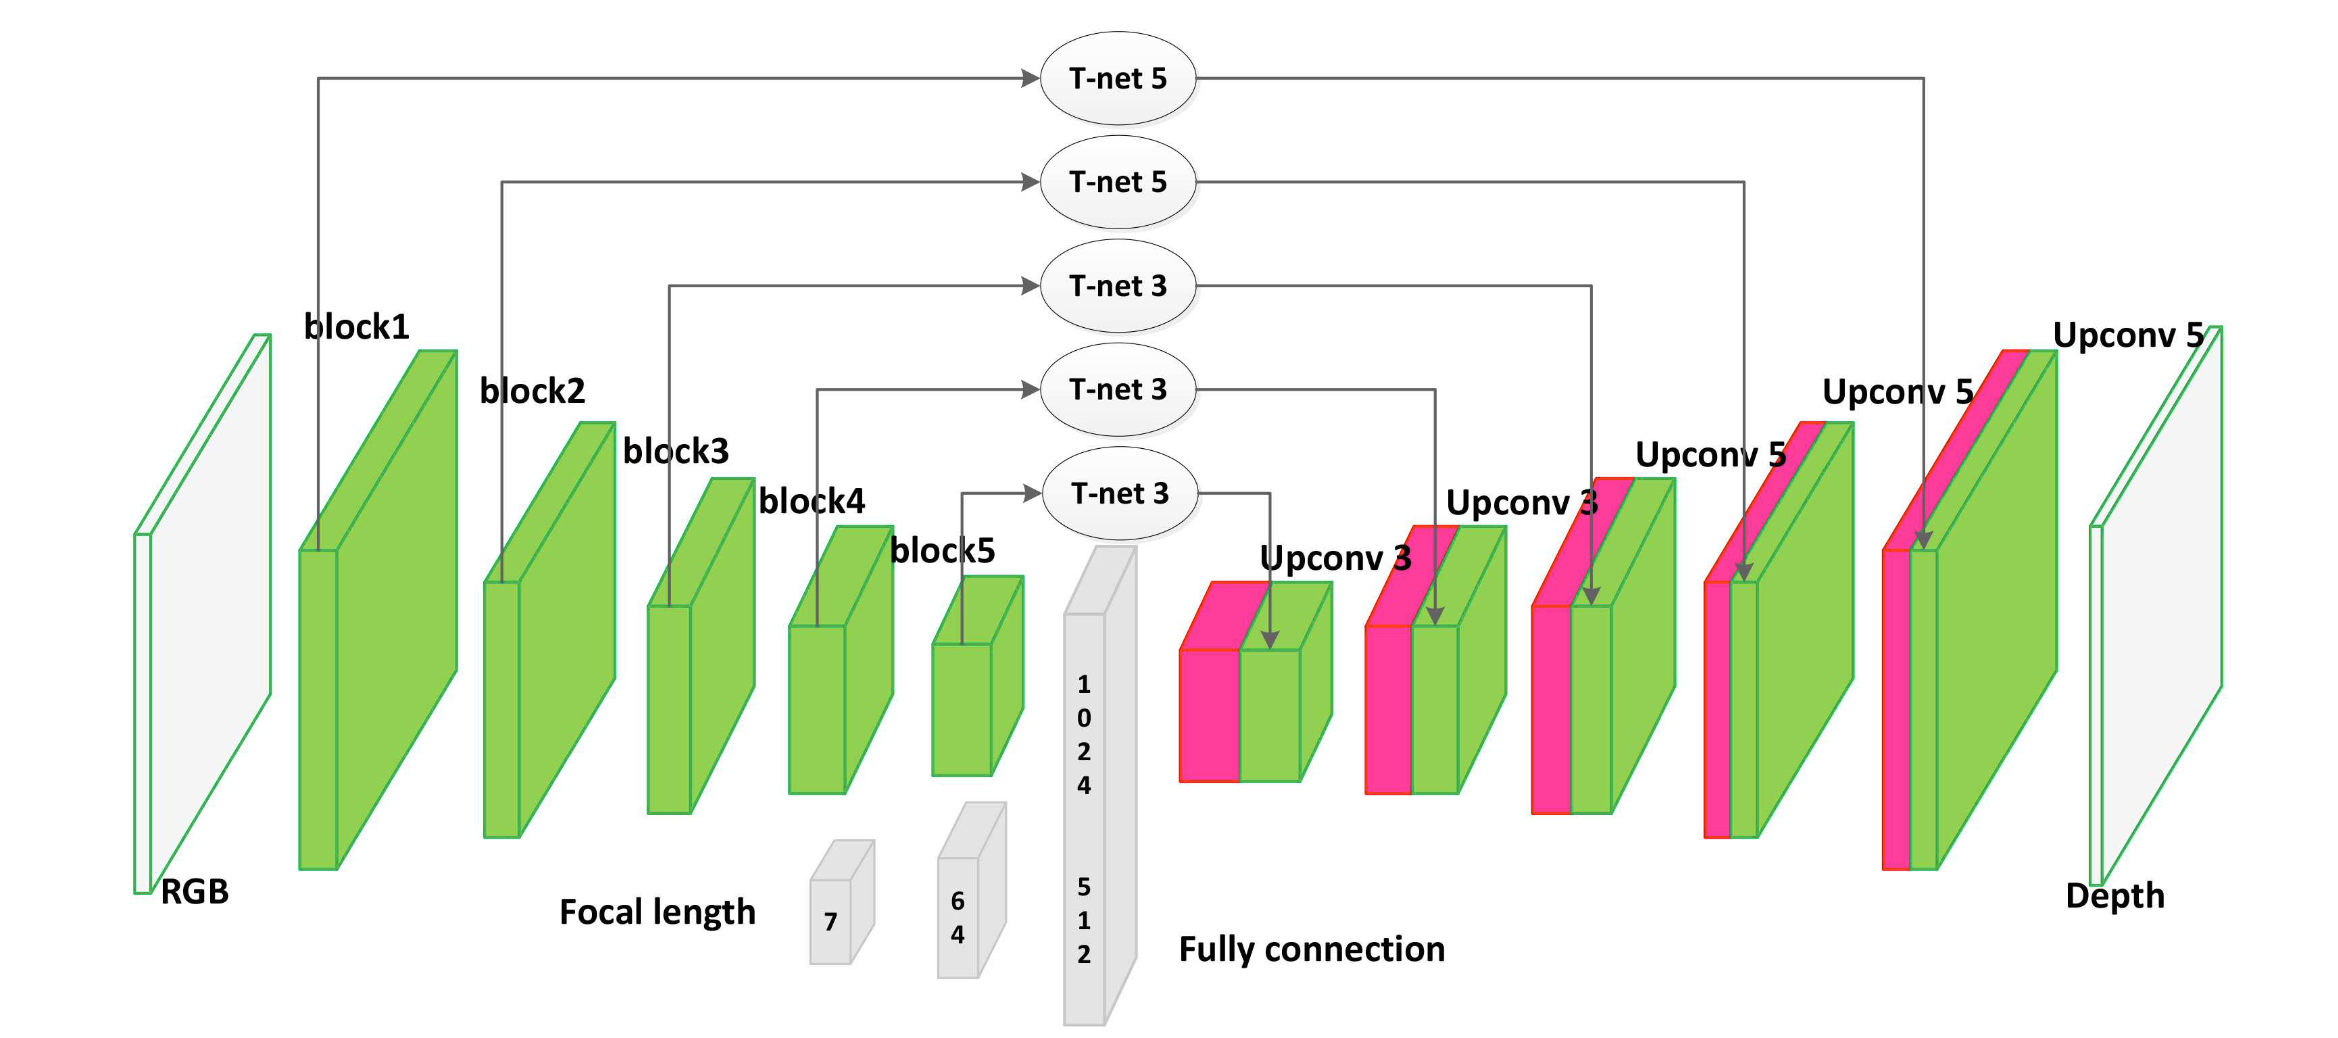
\includegraphics[width=0.5\textwidth]{Figs/FocalDLPicAr.png}
% \end{center}
% \caption{Architecture introduced by \cite{FocalDL} where focal length is taken as an input}
% \label{FocalDLPicAr}
% \end{figure}
%%%%%%%%%%%%%%%%%%%%%%



In popular datasets for depth perception, such as NYU Depth V2 and ScanNet, only a single image is captured per scene, and images with varying focal lengths are not available. However, in the approach proposed by \cite{FocalDL}, they generate images with different focal lengths by applying matrix operations to the original image. Figure \ref{FocalDLPicCMP} showcases two images with distinct focal lengths captured at the same scene. Subsequently, these newly generated images are passed through their deep neural network (DNN) to obtain depth maps as outputs. The method presented by \cite{FocalDL} surpasses the performance of state-of-the-art models in terms of prediction accuracy.

% To cite images just copy and paste these
\begin{figure}[h]
\begin{center}
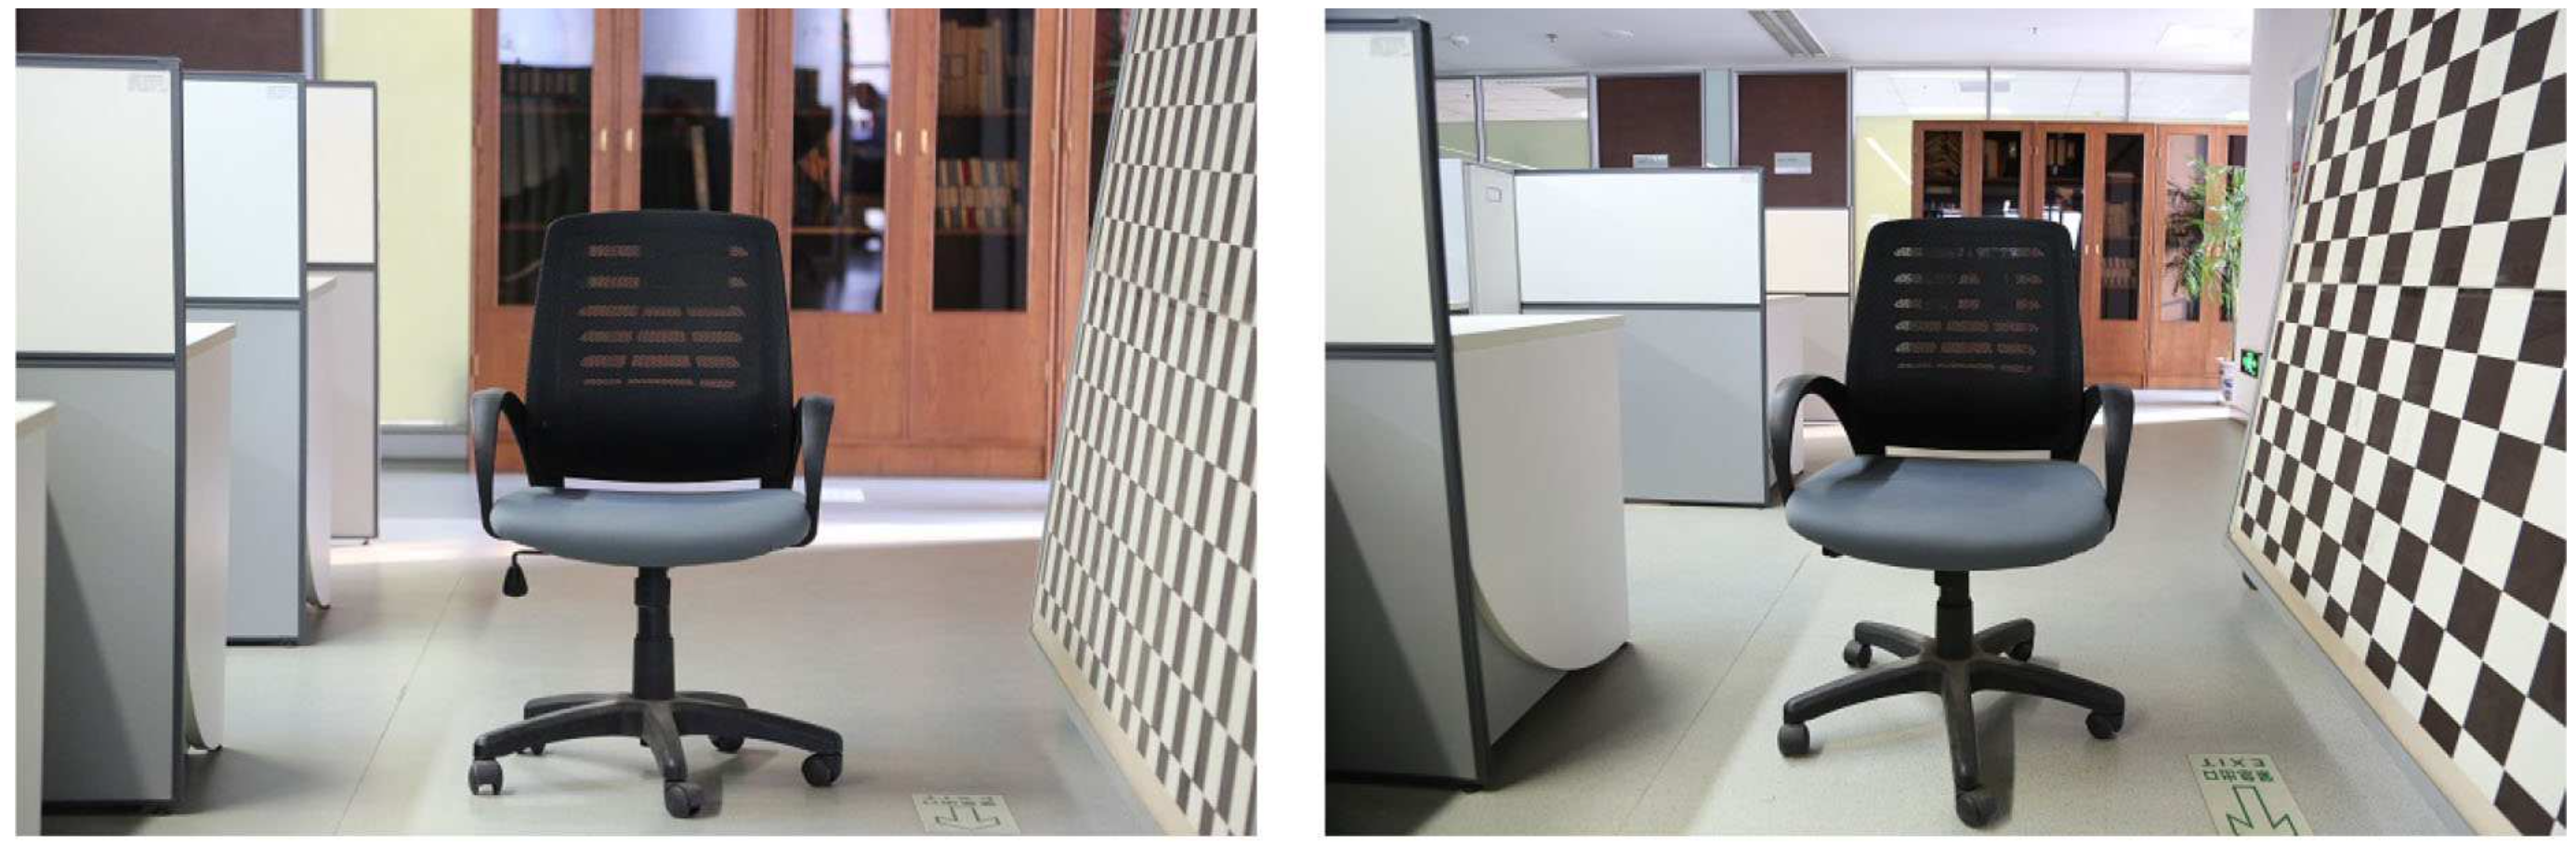
\includegraphics[width=0.6\textwidth]{Figs/FocalDLPicCMP.png}
\end{center}
\caption{Two pictures taken at the same place with cameras with different focal lengths}
\label{FocalDLPicCMP}
\end{figure}
%%%%%%%%%%%%%%%%%%%%%%

\subsection{Modular Depth Estimation from Single Indoor Images}

\cite{10.1007/978-3-030-11009-3_19} introduces a modular network architecture for estimating indoor scenes, which was adapted from the GAN (\cite{Gan2014}) and AlexNet (\cite{NIPS2012_4824}) architectures. In Figure \ref{Ito2019-figure}, the architecture initially takes an RGB image as input and passes it through the layout network $\displaystyle \mN_L$ and the object network $\displaystyle \mN_O$. The values obtained from $\displaystyle \mN_L$ and $\displaystyle \mN_O$ are then combined to determine a reliability score. If this score exceeds a certain threshold, the image data is further processed for depth estimation. Instead of solely learning features implicitly within the network, this architecture incorporates a \textit{discriminator network} that classifies each instance as either fake or real before proceeding to the depth estimation network.

% To cite images just copy and paste these
\begin{figure}[h]
\begin{center}
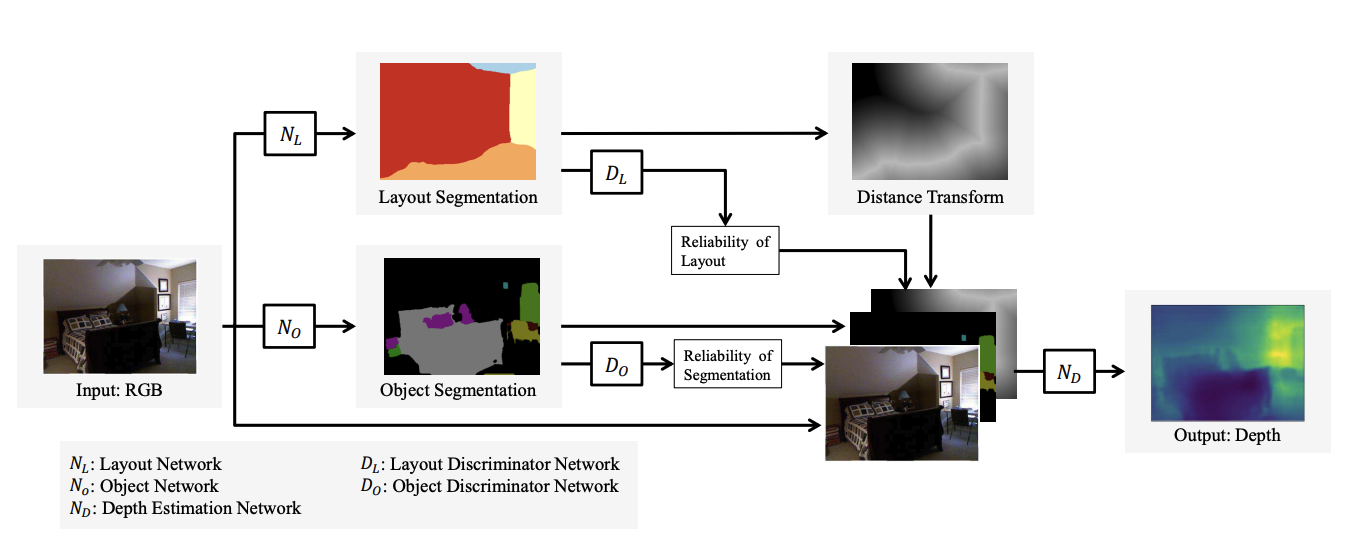
\includegraphics[width=0.6\textwidth]{Figs/Ito2019-figure.png}
\end{center}
\caption{Architecture of the system proposed by \citet{10.1007/978-3-030-11009-3_19}}
\label{Ito2019-figure}
\end{figure}
%%%%%%%%%%%%%%%%%%%%%%


\subsection{Different Model Architectures for learning-based approaches}

According to \cite{Masoumian}, depth estimation can be categorized into three divisions: monocular depth estimation (MDE), binocular depth (BDE), and multi-view depth estimation (MVDE). The earliest significant advancement in MDE, which involves estimating depth from a single viewpoint, can be traced back to a research paper from Stanford (\cite{Liu_2016}). Considering memory limitations, employing MDE is a suitable choice for deep learning (DL) applications on edge devices, as complex networks may not be practical for real-time applications. Architectures such as ResNet (\cite{He2015}) and DenseNet (\cite{huang2017densely}) strike a balance between accuracy and the power consumption requirements. Additionally, \cite{MobileNet2017} introduce MobileNet, a DNN architecture designed for low computational cost in mobile and embedded vision applications. Moreover, efficientNet proposed by \cite{tan2020efficientnet} outperforms ResNet and DenseNet in terms of computational cost, particularly when the image resolution is high \cite{Tadepalli}.


%%%%%%%%%%%%%%%%%%%%% Start of Section 3: Data Processing %%%%%%%%%%%%%%%%%%%%%

\section{Data Preprocessing}

Huggingface (\cite{huggingface}) offers a comprehensive collection of datasheets conveniently bundled in a library, providing convenient access. Therefore, the \cite{Silberman:ECCV12}'s /sayakpaul/nyu\_depth\_v2\   datasheet from Huggingface was chosen for its exceptional compilation of one of the largest image/depth datasets and its user-friendly interface. Upon closer inspection, the dataset reveals two distinct fields.

\begin{enumerate}
    \item Image : A PIL.PngImagePlugin.PngImageFile object with uint8 data type.
    \item Depth Map: A PIL.TiffImagePlugin.TiffImageFile object with float32 data type.
\end{enumerate}

\begin{minipage}{.5\textwidth}
    \centering
    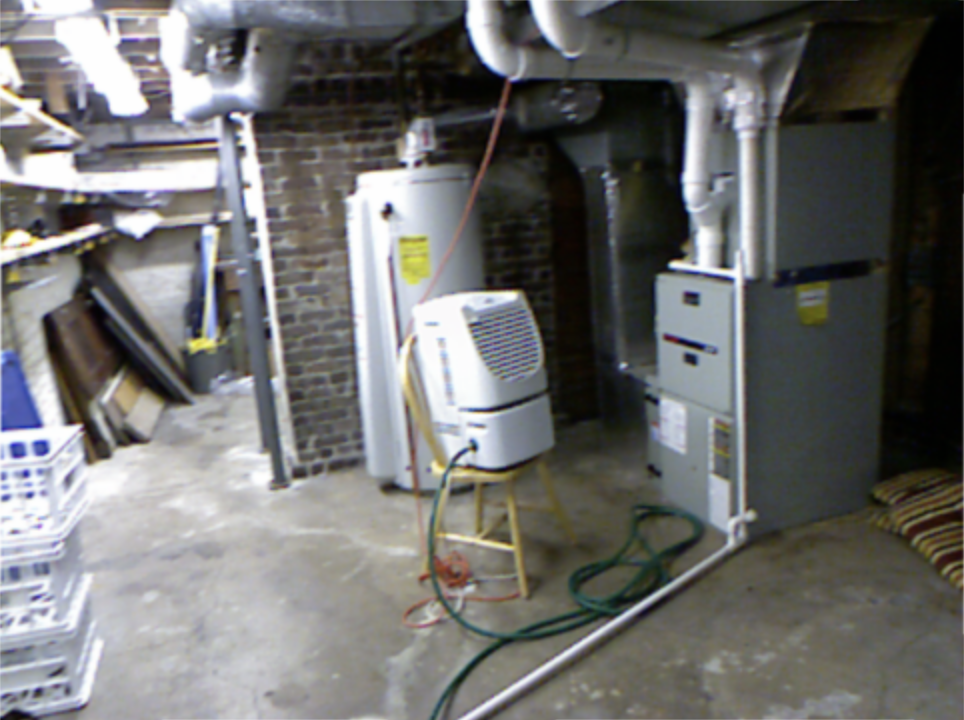
\includegraphics[width = 0.7\textwidth]{Figs/image.png}
    \captionof{figure}{Image}
    \label{image}
\end{minipage}%
\begin{minipage}{.5\textwidth}
    \centering
    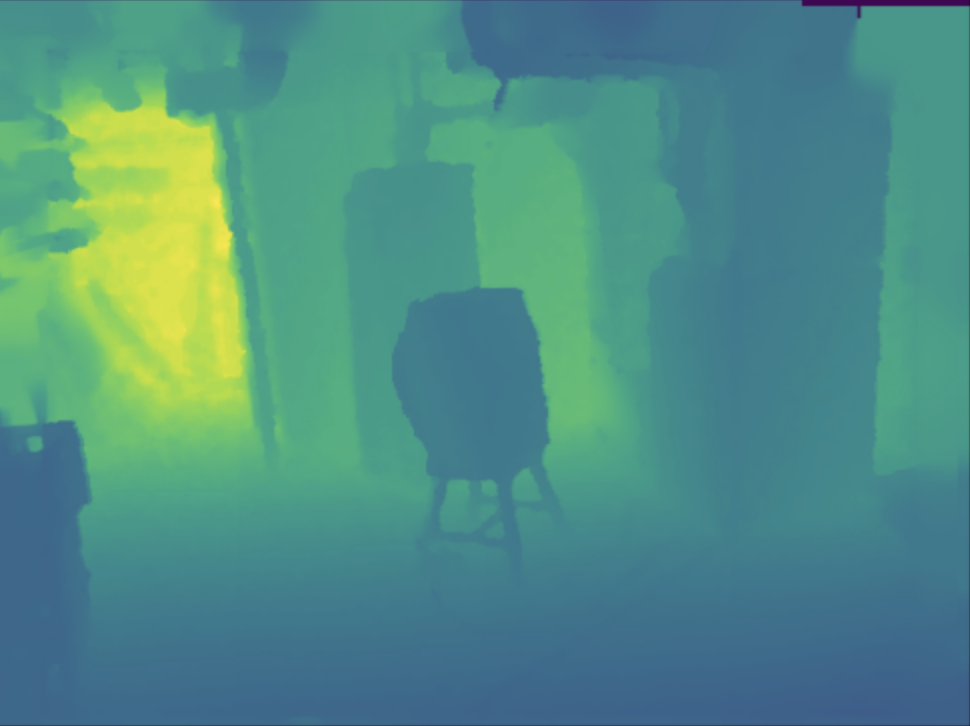
\includegraphics[width = 0.7\textwidth]{Figs/depth_map.png}
    \captionof{figure}{Depth map visualization}
    \label{depth_map}
\end{minipage}


Both datasets share a common resolution of 640 by 480. There is no need for data preprocessing in terms of resizing the data to a specific size. However, 
the following sections describe other data preprocessing steps that will be performed:

\subsection{Visualization}
To facilitate future debugging purposes, it would be beneficial to have a visualization of the depth map. Therefore, our team plans to devise a visualization mechanism for depth maps as part of the data preprocessing procedure. The procedure will begin by normalizing the depth map within a range of 0 to 1. Subsequently, the depth map will be converted into a numpy array with an RGB representation, which will have a shape of 640 by 480 by 3. This conversion will be achieved using the plt.cm.viridis function. Finally, by multiplying the resulting array by 255, we will obtain the desired visualization of the depth map, as depicted in Figure \ref{depth_map}.


\subsection{Data Augmentation}
By utilizing data augmentation, we can effectively mitigate the risk of overfitting and enhance the robustness of our model. Therefore, we will generate an additional dataset by randomly selecting augmentations from a predefined list. These augmentations include operations such as horizontal flip, random cropping, brightness contrast adjustment, gamma adjustment, and saturation adjustment. Subsequently, we will apply these augmentations randomly to our collection of 2000 images and their corresponding depth maps, and stored the augmented results.



\subsection{Data organization}

The original dataset downloaded from Huggingface consists of over 100GB, making it impractical to use the entire dataset. After careful consideration, it has been decided that our project dataset will consist of the first 2000 images, which amounts to a more manageable size of 9.2GB. This decision takes into account the storage limitations of our device, as expanding the dataset beyond this size could risk a potential system crash.

A design choice has been made to store all files as numpy arrays, as these files essentially contain 2D array information represented in various forms. By adopting a universal data type, significant future efforts can be saved.

The data has been organized into 5 folders: “image”, “depth\_map”, “depth\_map\_visualization”, “augmented\_image” and “augmented\_depth\_map.” Each folder contains the corresponding data. We have adopted a straightforward naming convention, for example: image\_17.npy and depth\_map\_17.npy, where the number represents the index of the data.


%%%%%%%%%%%%%%%%%%%%% Start of Section 4: Model Architecture %%%%%%%%%%%%%%%%%%%%%



\section{Model Architecture}
% \label{headings}
In this section, we present the overall architecture of our project, along with the model architectures for object detection and depth map generation.

\subsection{Overall Project Architecture}
Our overall project architecture comprises an object detector, a depth map generator, and a text-to-speech converter. The object detector is responsible for detecting objects in the image, labeling them, and creating bounding boxes around them. The depth map generator takes the original images as input and generates corresponding depth maps. We then combine the image with the bounded objects and its depth map. This allows us to establish a one-to-one relationship between detected objects and their distances. Various algorithms can be employed to calculate this distance, such as averaging all depth points or considering the average of the closest 25\% of depth points. The object's relative distance is determined based on its X and Y position in the image, as well as its actual distance. We use a text-to-speech converter to output the type of object, its distance, and its relative location. A visual representation of our project architecture is depicted in Figure \ref{Project Architecture}.

\begin{figure}[h]
\begin{center}
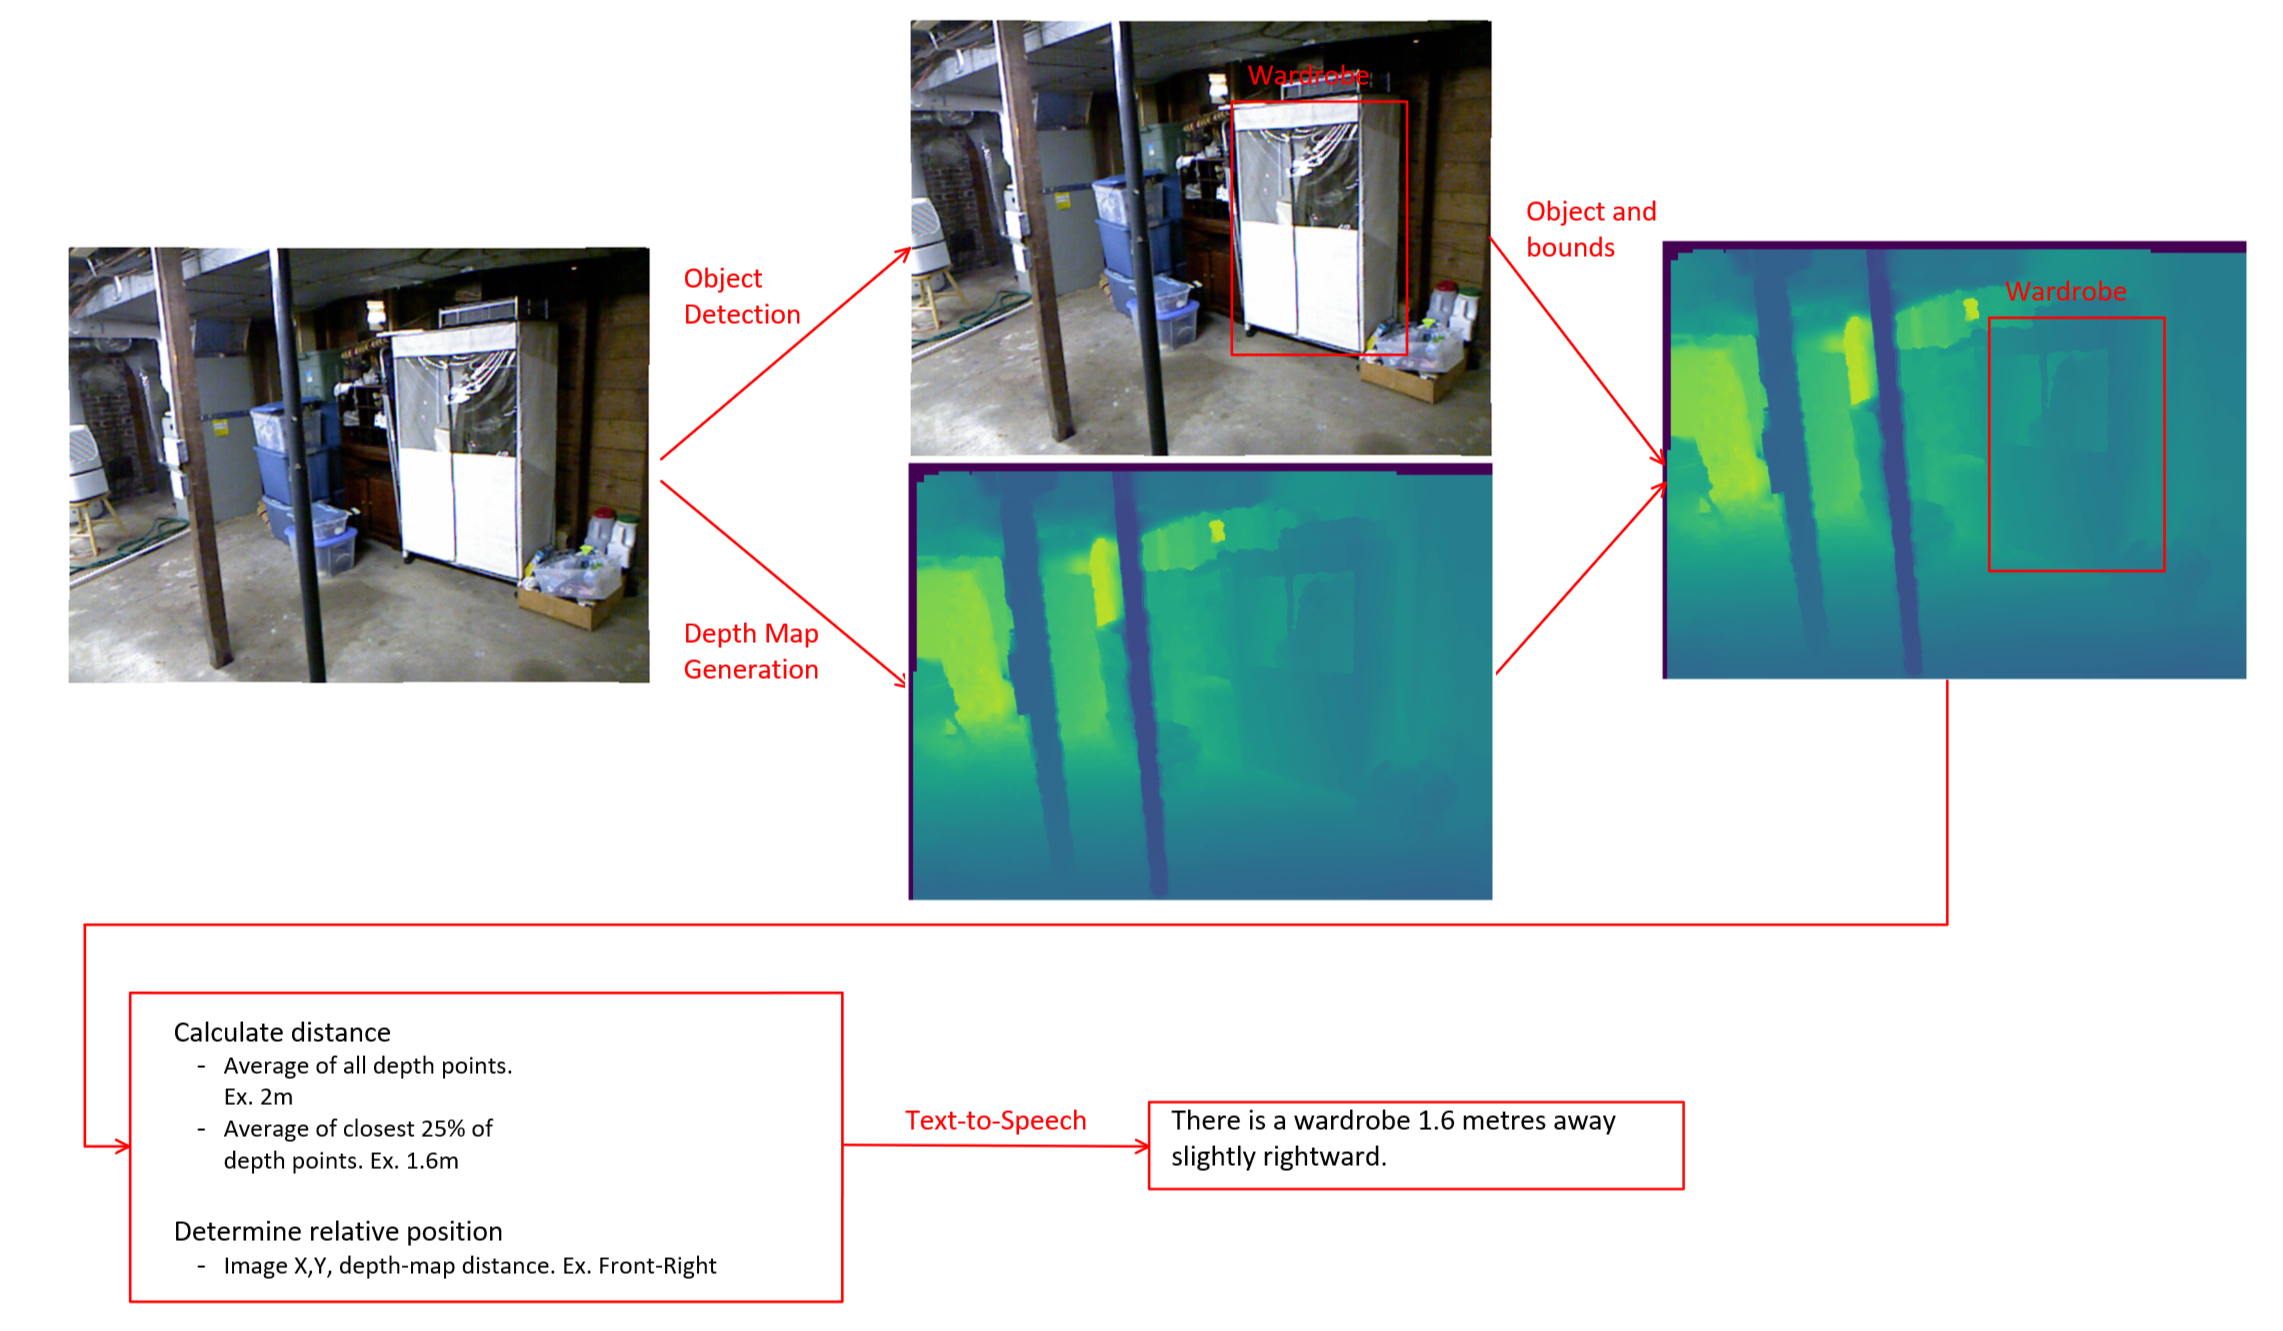
\includegraphics[width=1\textwidth]{Figs/Project Architecture.png}
\end{center}
\caption{Visual representation of the project architecture. (\cite{Silberman:ECCV12})}
\label{Project Architecture}
\end{figure}

\subsection{Object Detection Architecture}

We will utilize Convolutional Neural Networks (CNNs) for training the object detection model, taking inspiration from successful architectures like ResNet \cite{He2015} and AlexNet \cite{NIPS2012_4824}. Specifically, we will enhance the ResNet architecture, originally designed for image classification on ImageNet, to incorporate object detection capabilities with bounding box generation. Through modifications and the inclusion of additional layers and techniques, our goal is to empower the model to effectively detect objects and generate accurate bounding box predictions.


\subsection{Depth Map Generation Architecture}

Our plan involves utilizing U-Net \cite{RFB15a} for generating depth maps from input images. U-Net is a fast model that supports end-to-end training, even with small datasets. Additionally, we are considering replacing the encoder of U-Net with the DenseNet \cite{huang2017densely} or ResNet \cite{He2015} architecture to achieve more accurate results while preserving efficiency.



%%%%%%%%%%%%%%%%%%%%% Start of Section 5: Baseline %%%%%%%%%%%%%%%%%%%%%



\section{Baseline model}

We will use a support vector machine (SVM) as the baseline model for comparison with our neural network architecture. To begin, we will utilize the preprocessed dataset described in Section 3, which consists of two categories: RGB images paired with their corresponding depth map values, and labeled images representing different classes.

For image classification, we will create a hash table containing all the objects we aim to classify from the RGB images, using the preprocessed data mentioned earlier. Next, we will extract handcrafted features from the RGB images to capture relevant information, including color histograms, text descriptors, edge-based features, and geometric features. These extracted features will be normalized accordingly. Using the labeled images, we will train the SVM for multi-class classification by tuning the hyperparameters (such as the regularization parameter $\displaystyle C$ and kernel-specific parameters) through grid and random search. We will evaluate the accuracy of the SVM classification using metrics like root mean square or mean absolute error, both for training (roughly 75\% split) and validation sets (roughly 25\% split).

Similarly, for depth estimation, we will create a hash table containing the data objects and their corresponding regression values based on the preprocessed data. Handcrafted features (such as color histograms, text descriptors, edge-based features, and geometric features) will be extracted from the RGB images to capture relevant information. These features will be normalized, and class imbalance handling techniques will be applied if necessary. The SVM will be trained for multi-class classification using labeled images with values in a specific range. Hyperparameters will be tuned, and a suitable kernel function (such as linear or polynomial) will be selected through grid and random search. Accuracy evaluation for SVM regression will be performed using metrics like root mean square or mean absolute error, again for both training (roughly 75\% split) and validation sets (roughly 25\% split).

Finally, we will compare the accuracy of the SVM with our deep learning model to determine if our deep neural network outperforms the traditional machine learning approach. This evaluation will provide insights into the relative strengths of each method for both image classification and depth estimation tasks.



%%%%%%%%%%%%%%%%%%%%% Start of Section 6: Project Plan %%%%%%%%%%%%%%%%%%%%%



\section{Project Plan}

\subsection{ways of working and basic rules}
Since the group was formed, we have had several discussions on roles of team members. The detailed roles and responsibilities are reported in Table \ref{tab:teammember_table}. A Discord channel has been established for the group, where online meetings are held every Tuesday at 10 pm. Meetings with short notice, upon the request of team members, are discussed and scheduled through the Discord channel. A one-day advance notice is required for absences during the weekly meetings. However, the weekly meeting can be rescheduled or canceled in case of midterms or unforeseen circumstances.

We utilize a GitHub repository to store relevant codes and project resources. Git version control tools will be used to ensure smooth collaboration among team members without affecting each other's code. The following coding rules are in place:
\begin{itemize}
  \item After pushing, clear and concise commit messages, as well as comments in the code, are always required.
  \item For more complex feature developments, branches should be created.
  \item Only working code should be pushed, unless assistance is needed for debugging.

\end{itemize}

To manage tasks, we employ a group TODO list that is updated during the weekly meetings. The TODO list groups tasks into three categories based on their importance and urgency. Responsible members and deadlines are assigned based on task priority. High priority tasks are assigned to responsible team members with a deadline, typically within one week. Medium priority tasks are due within 1-2 weeks and may be moved to the high priority list as their deadlines approach. Medium priority tasks can be left without an assigned responsible member, but a deadline must still be set. Low priority tasks, such as personal background research, are also included in our TODO list, but they do not require a responsible member or a deadline. Table \ref{tab:timeline_table} presents our project timeline.

\begin{table}[h]
\centering
\begin{tabular}{|l|l|p{0.49\linewidth}|} \hline
Team Member & Role & Responsibilities \\ \hline
Jason Tai & Team Learder & Establish the structure of the overall project and its goals \\\hline
Rick Lin & Project Manager & Responsible for creating project plans, timelines, deliverables, and allocate DL/ML resources to the team \\ \hline
Danjie Tang & Data Management Lead & Lay the foundation for the group collaboration by preprocessing data in a speedy manner \\ \hline
Spencer Li & Architecture Lead & Carry on throughout research on state-of-art model architectures and provide insights on designing the model architecture for this project \\ \hline
\end{tabular}
\caption{\label{tab:teammember_table} Team members and corresponding responsibilities}
\end{table}


\begin{longtable}{|p{0.2\linewidth}|p{0.3\linewidth}|l|l|l|} \hline
    \centering
        Tasks: & ~ & Team member: & Deadline: & Done: \\ \hline
        Project Proposal & Create a google drive folder & Rick Lin & Jun 12 & Jun 12 \\ 
        (Hard deadline: & Create a github repo & Spencer Li & Jun 12 & Jun 12 \\ 
        Jun 16) & Abstract & Spencer / Jason & Jun 15 & Jun 14 \\ 
        ~ & Introduction & Jason & Jun 15 & Jun 14 \\ 
        ~ & Background \& Related Work & Rick / All & Jun 15 & Jun 16 \\ 
        ~ & Data processing & Danjie / Rick & Jun 15 & Jun 16 \\ 
        ~ & Model architecture & Spencer / Jason & Jun 15 & Jun 15 \\ 
        ~ & Baseline model & Rick & Jun 15  & Jun 15 \\ 
        ~ & Project plan & All & Jun 15  & Jun 16 \\ 
        ~ & Ethical consideration & Rick & Jun 15 & Jun 16 \\ 
        ~ & Risk register & All & Jun 15  & Jun 15 \\ 
        ~ & Illustration / Figure & All & Jun 15  & Jun 16 \\ \hline
        Data Processing & Processing scripts & Danjie & Jun 19 & ~ \\ \hline
        Object Detection Implementation& Model Implementation and initial test & Spencer / Rick & Jul 1 & ~ \\ 
        ~ & Model training and parameter tuning & All & Jul 8 & ~ \\ 
        ~ & Final testing & Spencer / Rick & Jul 10 & ~ \\ \hline
        Depth Perception Implementation& Model Implementation and initial test & Jason / Danjie & Jul 8 & ~ \\ 
        ~ & Model training and parameter tuning & All & Jul 15 & ~ \\ 
        ~ & Final testing & Jason / Danjie & Jul 17 & ~ \\ \hline
        Project Process Report (Hard deadline: Jul 14)& Tasks and deadlines to be set & All & Jul 6 & ~ \\ \hline
        % Report (Hard  & Notable contributions & ~ & Jul 13 & ~ \\ 
        % deadline: Jul 14) & Summary & ~ & Jul 13 & ~ \\ \hline
        Model Combining & Model combining & Spencer / Rick & Jul 19 & ~ \\
        and Audio Output & Audio generation & Danjie / Jason & Jul 19 & ~ \\
        Generation & System final test & All & Jul 23 & ~ \\ \hline
        Project Presentation Video (Hard & Brainstroming and individual script writing & All & Jul 27 & ~ \\ 
        deadline: Aug 4)& Script combining and finalizing & All & Jul 28 & ~ \\ 
        ~ & Video Recording & All & Aug 1 & ~ \\ 
        ~ & Final video editing and extra clips recording & All & Aug 3 & ~ \\  \hline
        Project Final Report (Hard deadline: Aug 11) & Tasks and deadlines to be set & All & Aug 4 & ~ \\  \hline
\caption{\label{tab:timeline_table} Project timeline}
\end{longtable}



\subsection{Measures of Success}
We have determined the measures of success of our model such that; the resulting program describes the room well enough such that it gives the user a rough idea of where objects in the room are, and our model outperforms the baseline model (SVM) in accuracy and recall, with a lower Root Mean Squared Error (RMSE) as well.


%Please add the following packages if necessary:
%\usepackage{booktabs, multirow} % for borders and merged ranges
%\usepackage{soul}% for underlines
%\usepackage[table]{xcolor} % for cell colors
%\usepackage{changepage,threeparttable} % for wide tables
%If the table is too wide, replace \begin{table}[!htp]...\end{table} with
%\begin{adjustwidth}{-2.5 cm}{-2.5 cm}\centering\begin{threeparttable}[!htb]...\end{threeparttable}\end{adjustwidth}







%%%%%%%%%%%%%%%%%%%%% Start of Section 7: Ethical %%%%%%%%%%%%%%%%%%%%%



\section{Ethical Considerations}
When developing our project for visually impaired individuals using deep learning, several critical ethical considerations must be addressed and carefully considered.

\subsection{Privacy of Individuals}
During the training of our deep learning model, the data used may contain sensitive information about individuals, such as location information and personal belongings. It is crucial for us to comply with relevant privacy regulations and guidelines, such as GDPR(General Data Protection Regulation) and PIPEDA(Personal Information Protection and Electronic Documents Act), to ensure robust measures are in place to protect the privacy of individuals (\cite{gdpr}, \cite{pipeda}).

\subsection{Data Security, Consent, and Usage}
Prior to training our model, it is essential to ensure that there is no unauthorized access or use of the data. Storing images in secure storage systems and preventing unauthorized access to storage areas are critical measures to uphold data security. Additionally, it is important to review the privacy policies regarding data collection in our dataset, ensuring that informed consent is obtained regarding data sharing and usage.

\subsection{Deployment and Representational Biases}
If the Object Detection and Depth Perception System designed to assist visually impaired individuals is deployed exclusively in affluent neighborhoods or areas with better infrastructure, either due to data bias or other considerations, it can result in biased outcomes and limit the benefits of the system for marginalized communities. Similarly, if the training data used for the system exhibits bias towards a particular group, it can lead to lower accuracy when detecting individuals from different ethnic backgrounds. It is crucial to address these biases and strive for fair and unbiased representation in our system.



%%%%%%%%%%%%%%%%%%%%% Start of Section 8: Risk Register %%%%%%%%%%%%%%%%%%%%%

\section{Risk Register}
Throughout the development of our project, it is crucial to carefully consider and address the following potential risk factors that may arise.

\subsection{Group Member Drops the Course}
If a group member decides to drop the course due to personal reasons or unforeseen circumstances, it is important for the member to communicate with the rest of the team before dropping. The member should discuss their intentions with the team, and the remaining members will assess the workload distribution. Depending on the circumstances, adjustments may need to be made to ensure that the remaining members can handle the additional responsibilities.

\subsection{Models Take Longer Than Expected}
If the selected models exceed the team's original time expectations, several measures can be taken to address the situation. Firstly, the team may consider leveraging GPU acceleration by utilizing available GPU devices or exploring the purchase of GPU accelerators such as NVIDIA Graphics Cards. In cases where the model architecture proves to be highly complex, it is advisable for our team to reevaluate the hyperparameters and explore optimization techniques as needed. Techniques like early stopping or transfer learning can be applied during the model training process to mitigate lengthy training times. Early stopping helps prevent unnecessary iterations when further performance improvements are unlikely, while transfer learning leverages pre-trained models for specific tasks, significantly reducing development time. By considering these strategies, our team can effectively manage and overcome challenges related to longer model training times.

\subsection{Changing Project Requirements}
If any changes to the project requirements are proposed during the development, whether small or significant, it is crucial for team members to communicate within the team to ensure clear understanding of the reasons behind the modifications. It is essential to reassess the necessity of changes, taking into account the project's overall objectives and feasibility. In cases where the chosen model proves to be excessively complex or encounters training difficulties, the team should discuss with TAs or the professor to evaluate the model's performance and select the most optimal course of action. Their expertise can help identify potential solutions, such as adjusting the model architecture, fine-tuning hyperparameters, or exploring alternative approaches.

\subsection{Intellectual Data Violation}
If any intellectual data violation occurs during the model training process, the team must reassess data sources and license usage terms. It is necessary to replace any inappropriate data with suitable alternatives and update the model training accordingly. Ensuring compliance with intellectual property rights is crucial to maintain ethical and legal standards.


% \subsubsection*{Author Contributions}
% If you'd like to, you may include  a section for author contributions as is done
% in many journals. This is optional and at the discretion of the authors.

% \subsubsection*{Acknowledgments}
% Use unnumbered third level headings for the acknowledgments. All
% acknowledgments, including those to funding agencies, go at the end of the paper.

\label{last_page}

\newpage
\bibliography{APS360_ref}
\bibliographystyle{iclr2022_conference}

\section*{Code access}

Link to GitHub repository: \url{https://github.com/Spencer-16/APS360-ToBeNamed}

\end{document}

